\documentclass[a4paper,12pt]{article}
\usepackage{a4wide}
\usepackage{pst-circ}
\usepackage{tikz}
\usetikzlibrary{calc}

\begin{document}
\pagestyle{empty}
\setlength{\parindent}{0em}

% c for custom
\newcommand{\cand}[9]{\logicand[ninputs=4,iec=true,bubblesize=0.1,inputa=#1,inputb=#2,inputc=#3,inputd=#4, ,invertinputa=#5,invertinputb=#6,invertinputc=#7,invertinputd=#8,invertoutput=#9]}

\newcommand{\cor}[9]{\logicor[ninputs=4,iec=true,bubblesize=0.1,inputa=#1,inputb=#2,inputc=#3,inputd=#4, ,invertinputa=#5,invertinputb=#6,invertinputc=#7,invertinputd=#8,invertoutput=#9]}

\newcommand{\cxor}[9]{\logicxor[ninputs=4,iec=true,bubblesize=0.1,inputa=#1,inputb=#2,inputc=#3,inputd=#4, ,invertinputa=#5,invertinputb=#6,invertinputc=#7,invertinputd=#8,invertoutput=#9]}


\section*{Basic Gates}
Your task is to program the behavior of an entity called "gates". This entity is declared in the attached file "gates.vhdl" and has the following properties:

\begin{itemize}
\item Inputs: A, B, C, D with type std\_logic
\item Outputs: O with type std\_logic
\end{itemize}

\begin{center}
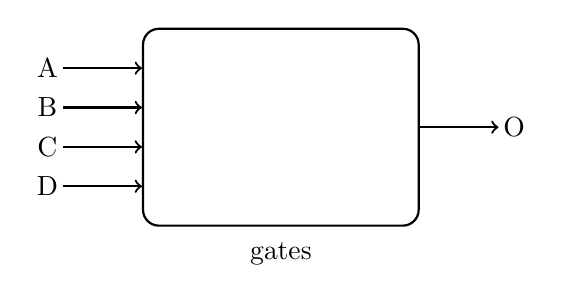
\begin{tikzpicture}
\draw node [draw,rectangle, minimum height=25mm, minimum width=35mm,rounded corners=2mm,thick](entity){};
\draw[->,thick] ($ (entity.west)-(10mm,7.5mm)$) -- ($ (entity.west) - (0mm,7.5mm)$);
\draw node at ($ (entity.west)-(12mm,7.5mm)$){D};
\draw[->,thick] ($ (entity.west)-(10mm,2.5mm)$) -- ($ (entity.west) - (0mm,2.5mm)$);
\draw node at ($ (entity.west)-(12mm,2.5mm)$){C};
\draw[->,thick] ($ (entity.west)-(10mm,-2.5mm)$) -- ($ (entity.west) - (0mm,-2.5mm)$);
\draw node at ($ (entity.west)-(12mm,-2.5mm)$){B};
\draw[->,thick] ($ (entity.west)-(10mm,-7.5mm)$) -- ($ (entity.west) - (0mm,-7.5mm)$);
\draw node at ($ (entity.west)-(12mm,-7.5mm)$){A};

\draw[->,thick] (entity.east) -- ($ (entity.east) + (10mm,0)$);;
\draw node at ($ (entity.east) + (12mm,0)$){O};

\draw node at ($ (entity) - (0,16mm)$){gates};

\end{tikzpicture}
\end{center}

Do not change the file "gates.vhdl"!
\\

The "gates" entity shall behave according to the following gate network:

\vspace{0.3cm}

\begin{center}
\psset{unit=0.9}
\begin{pspicture}(12,13)
%\psgrid
\psset{dotsize=0.15}

%input gates
%<b> =true/false
%       inputs enabled(a-d)  inputs negates(a-d)  output negated
%\<type> {<b>}{<b>}{<b>}{<b>} {<b>}{<b>}{<b>}{<b>} {<b>}(2,1){G0}
%\<type> {<b>}{<b>}{<b>}{<b>} {<b>}{<b>}{<b>}{<b>} {<b>}(2,4){G1}
%\<type> {<b>}{<b>}{<b>}{<b>} {<b>}{<b>}{<b>}{<b>} {<b>}(2,7){G2}
%\<type> {<b>}{<b>}{<b>}{<b>} {<b>}{<b>}{<b>}{<b>} {<b>}(2,10){G3}

%\<type> {<b>}{<b>}{<b>}{<b>} {<b>}{<b>}{<b>}{<b>} {<b>}(7,5.5){G4}

{{G0}} {{ IE0  }}{{ IE1  }}{{ IE2  }}{{ IE3  }} {{ IN0  }}{{ IN1  }}{{ IN2  }}{{ IN3  }} {{ ON0 }}(2,1){G0}
{{G1}} {{ IE4  }}{{ IE5  }}{{ IE6  }}{{ IE7  }} {{ IN4  }}{{ IN5  }}{{ IN6  }}{{ IN7  }} {{ ON1 }}(2,4){G1}
{{G2}} {{ IE8  }}{{ IE9  }}{{ IE10 }}{{ IE11 }} {{ IN8  }}{{ IN9  }}{{ IN10 }}{{ IN11 }} {{ ON2 }}(2,7){G2}
{{G3}} {{ IE12 }}{{ IE13 }}{{ IE14 }}{{ IE15 }} {{ IN12 }}{{ IN13 }}{{ IN14 }}{{ IN15 }} {{ ON3 }}(2,10){G3}

%output gate
{{G4}} {true}{true}{true}{true} {{ IN19 }}{{ IN18 }}{{ IN17 }}{{ IN16 }} {{ ON4 }}(7,5.5){G4}


%input lines and text
\psline{-}(0.4,12.4)(0.4,1.25)
\psline{-}(0.8,12.4)(0.8,1.25)
\psline{-}(1.2,12.4)(1.2,1.25)
\psline{-}(1.6,12.4)(1.6,1.25)
\rput(0.4,12.65){A}
\rput(0.8,12.65){B}
\rput(1.2,12.65){C}
\rput(1.6,12.65){D}

%output
\rput(10.8,6.5){O}

%lines input->gates, go=gateoffset
%\psline{*-}(1.6,go+0.25)(2,go+0.25)   %d
%\psline{*-}(1.2,go+0.75)(2,go+0.75)   %c
%\psline{*-}(0.8,go+1.25)(2.1,go+1.25) %b
%\psline{*-}(0.4,go+1.75)(2.1,go+1.75) %a

%G0 go=1
{{GI0}}   \psline{*-}(0.4,2.75)(2.1,2.75)%a
{{GI1}}   \psline{*-}(0.8,2.25)(2.1,2.25)%b
{{GI2}}   \psline{*-}(1.2,1.75)(2,1.75)%c
{{GI3}}   \psline{*-}(1.6,1.25)(2,1.25)%d

%G1 go=4
{{GI4}}  \psline{*-}(0.4,5.75)(2.1,5.75) %a
{{GI5}}   \psline{*-}(0.8,5.25)(2.1,5.25) %b
{{GI6}}   \psline{*-}(1.2,4.75)(2,4.75)   %c
{{GI7}}   \psline{*-}(1.6,4.25)(2,4.25)   %d

%G2 g0=7
{{GI8}}   \psline{*-}(0.4,8.75)(2.1,8.75) %a
{{GI9}}   \psline{*-}(0.8,8.25)(2.1,8.25) %b
{{GI10}}  \psline{*-}(1.2,7.75)(2,7.75)   %c
{{GI11}}  \psline{*-}(1.6,7.25)(2,7.25)   %d

%G3 go=10\\
{{GI12}} \psline{*-}(0.4,11.75)(2.1,11.75) %a
{{GI13}} \psline{*-}(0.8,11.25)(2.1,11.25) %b
{{GI14}} \psline{*-}(1.2,10.75)(2,10.75)   %c
{{GI15}} \psline{*-}(1.6,10.25)(2,10.25)   %d


%G0 to G4
\psline{-}(5.25,2)(7,2)
\psline{-}(7,2)(7,5.75)

%G1 to G4
\psline{-}(5.5,5)(5.5,6.25)
\psline{-}(5.5,6.25)(7,6.25)

%G2 to G4
\psline{-}(5.5,6.75)(5.5,8)
\psline{-}(5.5,6.75)(7,6.75)


%G3 to G4
\psline{-}(5.25,11)(7,11)
\psline{-}(7,11)(7,7.25)

\end{pspicture}
\end{center}

This behavior has to be programmed in the attached file "gates\_beh.vhdl".
\\

In VHDL predefined entities can be used and connected to solve problems. Use the attached IEEE 1164 Gates to build the given gate network. 6 types of gate entities are defined: AND[N], NAND[N], OR[N], NOR[N], XOR[N], XNOR[N] where [N] is the number of Inputs. Inputs are labelled I1..I[N], the Output is labled O.
\\

So for example a NAND with 3 inputs would be NAND3 and have the inputs I1, I2 and I3 and the output O. The needed package to use these entities is already imported in the attached "gates\_beh.vhdl".
\\

To turn in your solution write an email to {{SUBMISSIONEMAIL}} with Subject "Result Task {{TASKNR}}" and attach your file "gates\_beh.vhdl".

\vspace{0.7cm}

Good Luck and May the Force be with you.

\end{document}
